%%%%%%%%%%%%%%%%%%%%%%%%%%%%%%%%%%%%%%%%%
% Friggeri Resume/CV
% XeLaTeX Template
% Version 1.0 (5/5/13)
%
% This template has been downloaded from:
% http://www.LaTeXTemplates.com
%
% Original author:
% Adrien Friggeri (adrien@friggeri.net)
% https://github.com/afriggeri/CV
%
% License:
% CC BY-NC-SA 3.0 (http://creativecommons.org/licenses/by-nc-sa/3.0/)
%
% Important notes:
% This template needs to be compiled with XeLaTeX and the bibliography, if used,
% needs to be compiled with biber rather than bibtex.
%
%%%%%%%%%%%%%%%%%%%%%%%%%%%%%%%%%%%%%%%%%

\documentclass[print]{friggeri-cv} % Add 'print' as an option into the square bracket to remove colors from this template for printing
\usepackage{fontspec}
\usepackage{fontawesome}

\begin{document}

\header{James}{McCormac}{Curriculum Vitae} % Your name and current job title/field

%----------------------------------------------------------------------------------------
%	SIDEBAR SECTION
%----------------------------------------------------------------------------------------

\begin{aside} % In the aside, each new line forces a line break
\vspace{0.35cm}~
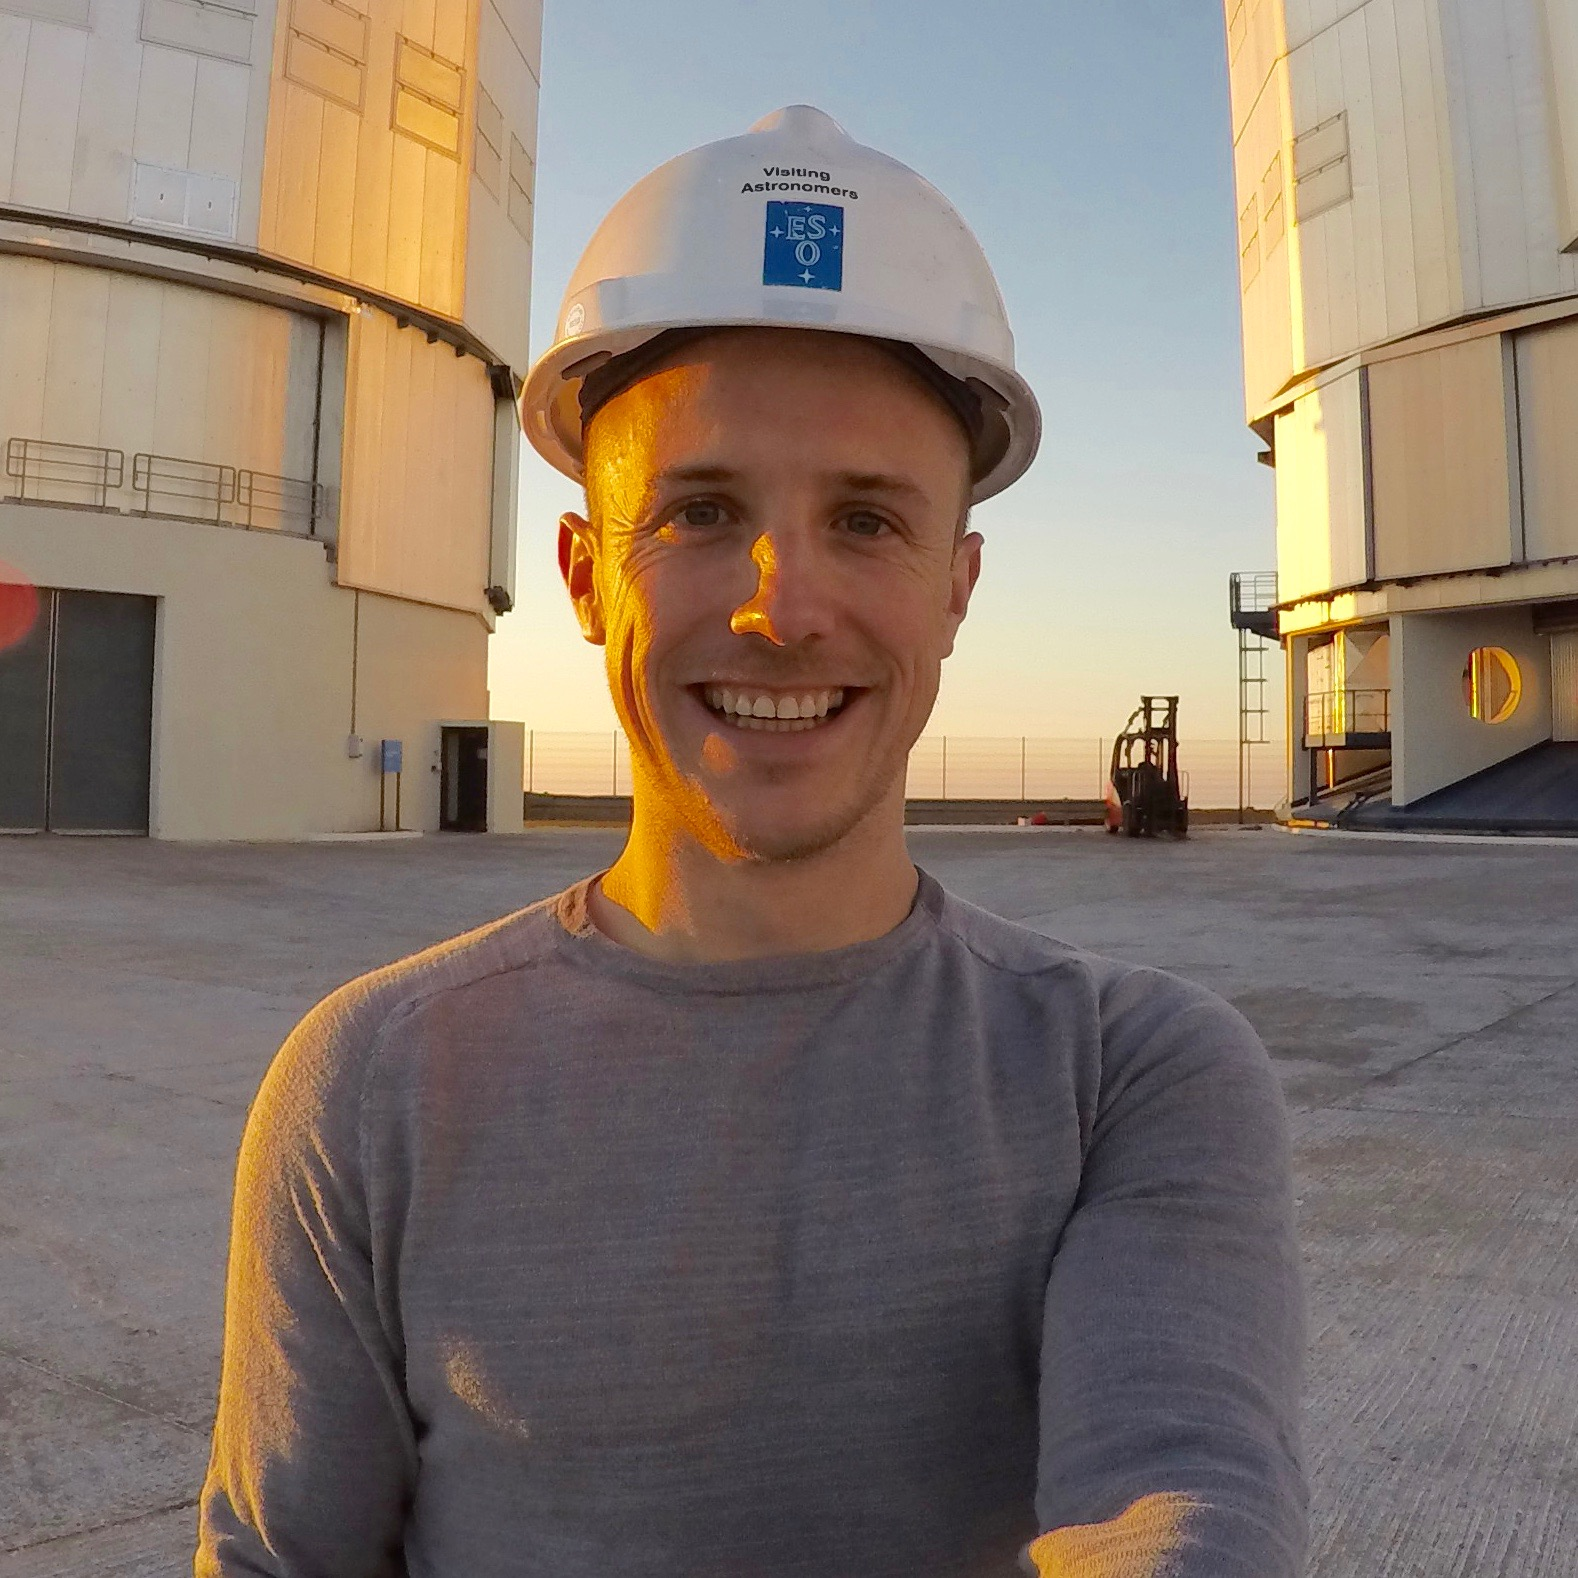
\includegraphics[width=4.0cm]{CV_Photo.jpg}\vspace{-0.5cm}
~
\section{Contact}
Department of Physics
University of Warwick
Gibbet Hill Road
Coventry
CV4 7AL
UK
~
\vspace{-0.2cm}{\bf Mobile:} 
+44 77139 46903
{\bf Office:} 
+44 24765 74211
{\bf Email:}
{\small j.j.mccormac@warwick.ac.uk}
~
\vspace{-0.5cm}\section{Links}
{\small \faLinkedin~jmcc001}
{\small \faGithub~\faSkype~jmccormac01}
{\small \faGlobe~jamesjmccormac.com}
~
\vspace{-0.5cm}\section{Languages}
English (Native)
Spanish (Fluent)
\section{Computing}
\vspace{1mm}{\bf Operating systems:} 
{\small Linux, macOS, Windows}
\vspace{1mm}{\bf Programming Languages:} 
{\small Python, C, Bash,\\HTML, CSS, Javascript}
\vspace{1mm}{\bf Web Frameworks:}
{\small Flask, JQuery}
\vspace{1mm}{\bf Databases:}
{\small MySQL}
\vspace{1mm}{\bf Grid Computing:} 
{\small SGE}
\vspace{1mm}{\bf Version Control:} 
{\small Git}
\vspace{1mm}{\bf Word Processing:} 
{\small \LaTeX, Microsoft Office}
\end{aside}

%----------------------------------------------------------------------------------------
%	EDUCATION SECTION
%----------------------------------------------------------------------------------------
%\vspace{0.5cm}
\section{Education}
\vspace{-0.8cm}
\begin{entrylist}
%------------------------------------------------
\entry
{}{}{Queen's University Belfast, BT7 1NN, U.K.}{}
%------------------------------------------------
\entry
{2008~--~2012}
{Doctor of Philosophy {\normalfont in Astronomy}}
{}{\vspace{-0.5cm}}
%------------------------------------------------
\entry
{2004~--~2008}
{Master of Science {\normalfont in Physics with Astrophysics with First Class Honours}}
{}{\vspace{-0.5cm}}
\end{entrylist}
%----------------------------------------------------------------------------------------
%	WORK EXPERIENCE SECTION
%----------------------------------------------------------------------------------------

\section{Experience}

\begin{entrylist}
%------------------------------------------------
\entry
{2014~--~2019}
{Department of Physics, University of Warwick}
{Gibbet Hill Road, Coventry, CV4 7AL}
{\emph{Postdoctoral Research Fellow: NGTS project, Cerro Paranal, Chile}\\
\vspace{-0.4cm}
 \begin{itemize}
 	\item Construction \& commissioning of a robotic observatory.
	\item Routine operation \& opto-mechanical maintenance of 12 telescopes.
	\item Development of operational software and environment monitoring.
	\item Development of observatory web interface in Python, Flask and MySQL.
	\item Development of web-based survey strategy tool (Javascript, HTML, CSS).
	\item Write \& maintain TWiki-based documentation.
	\item Exploitation of scientific results through exoplanet discoveries from \emph{NGTS}.
 \end{itemize}} 
 %------------------------------------------------
\entry
{2011~--~2018}
{Department of Physics, University of Warwick}
{Gibbet Hill Road, Coventry, CV4 7AL}
{\emph{NITES telescope manager, ORM, La Palma, Canary Islands, Spain}\\
\vspace{-0.4cm}
 \begin{itemize}
 	\item Construction \& commissioning of the semi-robotic observatory.
	\item Routine operation \& opto-mechanical maintenance of 0.4m telescope.
	\item Development of operational software and environment monitoring.
	\item High-precision photometric follow-up of \emph{SuperWASP} exoplanets.
	\item Provide training and support to postgraduate student users.
	\item Co-supervise masters projects -- characterising galactic stellar clusters.
	\item Data analysis of large survey for exoplanets in the globular cluster M71.
 \end{itemize}} 
%------------------------------------------------
\entry
{2015~--~2018}
{Department of Physics, University of Warwick}
{Gibbet Hill Road, Coventry, CV4 7AL}
{\emph{Python Programming Lab Demonstrator}\\
\vspace{-0.4cm}
 \begin{itemize}
 	\item Supervise practical lab sessions for 1$^{st}$ year Python programming course.
	\item Demonstrate basic operations and how to think programmatically.
	\item Demonstration of pseudo-code for sounding out initial ideas.
	\item Provide one-on-one support for students having difficulties.
 \end{itemize}} 
%------------------------------------------------
\entry
{2016~--~2018}
{Department of Physics, University of Warwick}
{Gibbet Hill Road, Coventry, CV4 7AL}
{\emph{Public Outreach: Warwick Astro Planetarium}\\
\vspace{-0.4cm}
 \begin{itemize}
 	\item Visit local primary schools with the department's inflatable IMAX-style planetarium and present a series of immersive videos on astronomy. 
	\item Interact with young children and answer questions about the universe. 
	\item Aim to engage with children and promote STEM subjects. 
 \end{itemize}}
%------------------------------------------------
\entry
{2012~--~2014}
{Isaac Newton Group of Telescopes}
{Santa Cruz de La Palma, Canary Islands, Spain}
{\emph{Telescope Operator \& Support Astronomer, 4.2m William Herschel Telescope}\\
\vspace{-0.4cm}
 \begin{itemize}
 	\item Was responsible for both ING telescopes for up to 100 nights per year.
	\item Provided expert training and support to visiting international astronomers.
	\item Was responsible for minimising technical downtime at the observatory.
	\item Routinely configured and calibrated the \emph{ACAM}, \emph{IDS}, \emph{LIRIS} \& \emph{WYFFOS} spectrographs, plus the \emph{ACAM}, \emph{PFIP} \& \emph{WFC} CCD cameras. 
	\item Developed Python scripts for efficient observing and data calibration.
 	\item Developed a Raspberry Pi driven auxiliary camera for the RoboDIMM astronomical seeing monitor.
\end{itemize}}
\end{entrylist}
\begin{entrylist}
%------------------------------------------------
\entry
{}
{}
{}
{
\vspace{-1cm}
 \begin{itemize}
	\item Supervised summer student project in 2013. The project was 50\% python programming: developing an automated calibration process for the ACAM imager; and 50\% science: measuring accurate colours for stars in the M71 globular cluster. 
	\item Completed multiple first-responder medical courses, driving safety, fire safety and general health \& safety courses, required for remote site work.
 \end{itemize}}  
%------------------------------------------------
\entry
{2008~--~2010}
{Queen's University Belfast}
{University Road, Belfast BT7 1NN}
{\emph{PhD Research Project: The Next Generation Transit Survey Prototype} \\
\vspace{-0.4cm}
 \begin{itemize}
 	\item Designed and built the prototype telescope for newly proposed transiting exoplanet survey \emph{NGTS}.
	\item Commissioned the prototype at the ORM, La Palma, Canary Islands, Spain and operated it remotely from my home at sea level on La Palma between 2009 and 2010.
	\item Developed a telescope, camera, focuser and dome control system in C.
	\item Analysed photometric data using Python and demonstrated the prototype's ability to detect super-Earth and Neptune-sized exoplanets. The commencement of the full �3M NGTS project was based in part on the results of this prototype.
\end{itemize}}
%------------------------------------------------
\entry
{2009~--~2010}
{Isaac Newton Group of Telescopes}
{Santa Cruz de La Palma, Canary Islands, Spain}
{\emph{Student Support Astronomer, 2.5m Isaac Newton Telescope} \\
\vspace{-0.4cm}
 \begin{itemize}
 	\item Provided expert training and support to visiting international astronomers.
	\item Configured the \emph{IDS} spectrograph and \emph{WFC} CCD camera as per the visiting astronomer's requirements. 
	\item Developed various Python scripts to automate observing and calibration tasks and increase the overall efficiency of the limited telescope time. 
	\item Provided technical feedback to visiting astronomers based on their telescope time application. 
\end{itemize}
}
%------------------------------------------------
\end{entrylist}

%----------------------------------------------------------------------------------------
%	AWARDS SECTION
%----------------------------------------------------------------------------------------

\section{Awards}

\begin{entrylist}
%------------------------------------------------
\entry
{2017}
{Performance Merit Award}
{University of Warwick}
{Award for excellent performance during previous 1.5 years}
\entry
{2013 \& 2014}
{Exceptional Performance Award}
{Isaac Newton Group of Telescopes}
{Award for exceptional performance in my position as Telescope Operator \& Support Astronomer at the ING.}
\entry
{2008~--~2011}
{Department of Employment \& Learning PhD scholarship}
{Queen's University Belfast}
{Funding for tuition fees and a stipend during a 3 year PhD degree.}
\entry
{2008}
{Raymond Greer Award}
{Queen's University Belfast}
{Awarded each year for the best overall MSci in Physics.}
\entry
{2008}
{Certificate of Entrepreneurial Studies}
{Queen's University Belfast}
{Awarded to the winners of an Entrepreneurial Studies competition.}
%------------------------------------------------
\end{entrylist}

%----------------------------------------------------------------------------------------
%	PUBLICATIONS SECTION
%----------------------------------------------------------------------------------------

\section{Publications}
{\bf First-author publications:}\\
~\vspace{-2mm}\\
\begin{entrylist}
\entry
{\small 2017}
{\small The Next Generation Transit Survey - Prototyping Phase}
{}
{\small McCormac, J., et al. 2017, PASP, 129, 972}
%------------------------------------------------
\entry
{\small 2014}
{\small A Search for Photometric Variability towards M71 with the Near-Infrared Transiting ExoplanetS Telescope}
{}
{\small McCormac, J., et al. 2014, MNRAS, 438, 3383}
%------------------------------------------------
\end{entrylist}
\begin{entrylist}
\entry
{\small 2013}
{\small DONUTS: A Science Frame Autoguiding Algorithm with Sub-Pixel Precision, Capable of Guiding on Defocused Stars}
{}
{\small McCormac, J., et al. 2013, PASP, 125, 548}
%------------------------------------------------
\end{entrylist}\\
%%%%%%%%%%%%%%%%%%%%%%%%
{\bf Co-authored publications:}\\
~\vspace{-2mm}\\
\begin{entrylist}
\entry
{\small 2018}
{\small Unmasking the hidden NGTS-3Ab: a hot Jupiter in an unresolved binary system}
{}
{\small G{\"u}nther, M.~N., et al. 2018, MNRAS, 478, 4720}
%------------------------------------------------
\entry
{\small 2018}
{\small Automatic vetting of planet candidates from ground-based surveys: machine learning with NGTS}
{}
{\small Armstrong, D. J., et al. 2018, MNRAS, 478, 4225}
%------------------------------------------------
\entry
{\small 2018}
{\small Ground-based detection of G star superflares with NGTS}
{}
{\small Jackman, J. A. G., et al. 2018, MNRAS, 477, 4655}
%------------------------------------------------
\entry
{\small 2018}
{\small SPECULOOS: a network of robotic telescopes to hunt for terrestrial planets around the nearest ultracool dwarfs}
{}
{\small Delrez, L., et al. 2018, SPIE submitted }
%------------------------------------------------
\entry
{\small 2018}
{\small An Earth-sized exoplanet with a Mercury-like composition}
{}
{\small Santerne, A., et al. 2018, Nature Astronomy, 2, 393}
%------------------------------------------------
\entry
{\small 2018}
{\small NGTS-2b: An inflated hot-Jupiter transiting a bright F-dwarf}
{}
{\small Raynard, L., et al. 2018, MNRAS submitted }
%------------------------------------------------
\entry
{\small 2018}
{\small The Next Generation Transit Survey (NGTS)}
{}
{\small Wheatley, P.~J., et al. 2018, MNRAS, 475, 4, 4476}
%------------------------------------------------
\entry
{\small 2018}
{\small NGTS-1b: A hot Jupiter transiting an M-dwarf}
{}
{\small Bayliss, D., et al. 2018, MNRAS, 475, 4, 4467}
%------------------------------------------------
\entry
{\small 2018}
{\small MASCARA-2 b. A hot Jupiter transiting the mV = 7.6 A-star HD 185603}
{}
{\small Talens, G. J. J., et al. 2018, A\&A, 612, A57}
%------------------------------------------------
\entry
{\small 2018}
{\small The discovery of WASP-151b, WASP-153b, WASP-156b: Insights on giant planet migration and the upper boundary of the Neptunian desert}
{}
{\small Demangeon, O. D. S., et al. 2018, A\&A, 610, A63}
%------------------------------------------------
\entry
{\small 2018}
{\small LRG-BEASTS III: ground-based transmission spectrum of the gas giant orbiting the cool dwarf WASP-80}
{}
{\small Kirk, J., et al. 2018, MNRAS, 474, 876}
%------------------------------------------------
\entry
{\small 2018}
{\small Qatar Exoplanet Survey: Qatar-6b?A Grazing Transiting Hot Jupiter}
{}
{\small Alsubai, K., et al. 2018, AJ, 155, 52}
%------------------------------------------------
\entry
{\small 2018}
{\small The First Post-Kepler Brightness Dips of KIC 8462852}
{}
{\small Boyajian, T. S., et al. 2018, ApJ, 853, L8}
%------------------------------------------------
\entry
{\small 2017}
{\small Centroid vetting of transiting planet candidates from the Next Generation Transit Survey}
{}
{\small Gunther, M., et al. 2017, MNRAS, 472, 295}
%------------------------------------------------
\entry
{\small 2017}
{\small MASCARA-1 b. A hot Jupiter transiting a bright m$_{V}$ = 8.3 A-star in a misaligned orbit}
{}
{\small Talens, G.~J.~J., et al. 2017, A\&A, 606, A73}
%------------------------------------------------
\entry
{\small 2017}
{\small A population of faint low surface brightness galaxies in the Perseus cluster core}
{}
{\small Wittmann, C., et al. 2017, MNRAS, 470, 1512}
%------------------------------------------------
\entry
{\small 2017}
{\small The EURONEAR Lightcurve Survey of Near Earth Asteroids}
{}
{\small Vaduvescu, O., et al. 2017, Earth Moon and Planets, 120, 41}
%------------------------------------------------
\entry
{\small 2017}
{\small Rayleigh scattering in the transmission spectrum of HAT-P-18b}
{}
{\small Kirk, J., et al. 2016, MNRAS, 468, 3907}
%------------------------------------------------
\entry
{\small 2017}
{\small K2-110 b: a massive mini-Neptune exoplanet}
{}
{\small Osborn, H. P., et al. 2017, A\&A, 604, A19}
%------------------------------------------------
\entry
{\small 2017}
{\small From Dense Hot Jupiter to Low Density Neptune: The Discovery of WASP-127b, WASP-136b and WASP-138b}
{}
{\small Lam, K.~W.~F., et al. 2017, A\&A, 599, A3}
%------------------------------------------------
\entry
{\small 2017}
{\small GRB 171205A: GOTO detection of the optical counterpart.}
{}
{\small Steeghs, D., et al. 2017, GRB Coordinates Network, Circular Service, No. 22190, \#1}
%------------------------------------------------
\end{entrylist}
\begin{entrylist}
\entry
{\small 2016}
{\small WASP-92b, WASP-93b and WASP-118b: three new transiting close-in giant planets}
{}
{\small Hay, K. L., et al. 2016, MNRAS, 463, 3276}
%------------------------------------------------
\entry
{\small 2016}
{\small The Astropy Problem}
{}
{\small Muna, D., et al. 2016, arXiv, 1610.03159}
%------------------------------------------------
\entry
{\small 2016}
{\small K2-30 b and K2-34 b: Two inflated hot Jupiters around solar-type stars}
{}
{\small Lillo-Box, J., et al. 2016, A\&A, 594, A50}
%------------------------------------------------
\entry
{\small 2016}
{\small WASP-113b and WASP-114b, two inflated hot Jupiters with contrasting densities}
{}
{\small Barros, S. C. C., et al. 2016, A\&A, 593, A113}
%------------------------------------------------
\entry
{\small 2016}
{\small The Next Generation Transit Survey Becomes Operational at Paranal}
{}
{\small West, R. G., et al. 2016, ESO Messenger, 165, 10}
%------------------------------------------------
\entry
{\small 2016}
{\small Supernova 2014J at M82 - II. Direct analysis of a middle-class Type Ia supernova}
{}
{\small Vallely, P., et al. 2016, MNRAS, 460, 1614}
%------------------------------------------------
\entry
{\small 2016}
{\small K2-29 b/WASP-152 b: An Aligned and Inflated Hot Jupiter in a Young Visual Binary}
{}
{\small Santerne, A., et al. 2016, ApJ, 824, 55}
%------------------------------------------------
\entry
{\small 2016}
{\small Single transit candidates from K2: detection and period estimation}
{}
{\small Osborn, H. P., et al. 2016, MNRAS, 427, 2273}
%------------------------------------------------
\entry
{\small 2016}
{\small SN 2014J at M82 - I. A middle-class Type Ia supernova by all spectroscopic metrics}
{}
{\small Galbany, L., et al. 2016, MNRAS, 457, 525}
%------------------------------------------------
\entry
{\small 2016}
{\small WASP-135b: A Highly Irradiated, Inflated Hot Jupiter Orbiting a G5V Star}
{}
{\small Spake, J. J., et al. 2016, PASP, 128, 2}
%------------------------------------------------
\entry
{\small 2016}
{\small K2 variable catalogue - II. Machine learning classification of variable stars and eclipsing binaries in K2 fields 0-4}
{}
{\small Armstrong, D. J., et al. 2016, MNRAS, 456, 2260}
%------------------------------------------------
\entry
{\small 2015}
{\small Photodynamical mass determination of the multiplanetary system K2-19}
{}
{\small Barros, S. C. C., et al. 2015, MNRAS, 454, 4267}
%------------------------------------------------
\entry
{\small 2015}
{\small Characterization of the K2-19 Multiple-transiting Planetary System via High-dispersion Spectroscopy, AO Imaging, and Transit Timing Variations}
{}
{\small Narita, N., et al. 2015, ApJ, 815, 47}
%------------------------------------------------
\entry
{\small 2015}
{\small One of the closest exoplanet pairs to the 3:2 mean motion resonance: K2-19b and c}
{}
{\small Armstrong, D. J., et al. 2015, A\&A, 582, A33}
%------------------------------------------------
\entry
{\small 2015}
{\small K2 Variable Catalogue: Variable stars and eclipsing binaries in K2 campaigns 1 and 0}
{}
{\small Armstrong, D. J., et al. 2015, A\&A, 579, A19}
%------------------------------------------------
\entry
{\small 2015}
{\small Subaru and Swift observations of V652 Herculis: resolving the photospheric pulsation}
{}
{\small Jeffery, C. S., et al. 2015, MNRAS, 447, 2836}
%------------------------------------------------
\entry
{\small 2014}
{\small The EBLM project. II. A very hot, low-mass M dwarf in an eccentric and long-period, eclipsing binary system from the SuperWASP Survey}
{}
{\small G{\'o}mez Maqueo Chew, Y., et al. 2014, A\&A, 572, A50}
%------------------------------------------------
\entry
{\small 2014}
{\small A window on exoplanet dynamical histories: Rossiter-McLaughlin observations of WASP-13b and WASP-32b}
{}
{\small Brothwell, R. D., et al. 2014, MNRAS, 440, 3392}
%------------------------------------------------
\entry
{\small 2013}
{\small Discovery of WASP-65b and WASP-75b: Two hot Jupiters without highly inflated radii}
{}
{\small Gomez Maqueo Chew, Y., et al. 2013, A\&A, 559, 36}
%------------------------------------------------
\entry
{\small 2013}
{\small WASP-54b, WASP-56b, and WASP-57b: Three new sub-Jupiter mass planets from SuperWASP}
{}
{\small Faedi, F., et al. 2013, A\&A, 551, A73}
%------------------------------------------------
\entry
{\small 2013}
{\small WASP-52b, WASP-58b, WASP-59b, and WASP-60b: Four new transiting close-in giant planets}
{}
{\small H{\'e}brard, G., et al. 2013, A\&A, 549, A134}
%------------------------------------------------
\entry
{\small 2012}
{\small A hot Uranus transiting the nearby M dwarf GJ 3470. Detected with HARPS velocimetry. Captured in transit with TRAPPIST photometry}
{}
{\small Bonfils, X., et al. 2012, A\&A, 546, A27}
%------------------------------------------------
\entry
{\small 2012}
{\small NGTS: a robotic transit survey to detect Neptune and super-Earth mass planets}
{}
{\small Chazelas, B., et al. 2012, SPIE, 8444, 84440E}
%------------------------------------------------
\end{entrylist}
\begin{entrylist}
\entry
{\small 2012}
{\small A transiting companion to the eclipsing binary KIC002856960}
{}
{\small Armstrong, D. J., et al. 2012, A\&A, 545, L4}
%------------------------------------------------
\entry
{\small 2011}
{\small WASP-35b, WASP-48b, and HAT-P-30b/WASP-51b: Two New Planets and an Independent Discovery of a Hat Planet}
{}
{\small Enoch, B., et al. 2011, AJ, 142, 86}
%------------------------------------------------
\entry
{\small 2011}
{\small WASP-40b: Independent Discovery of the 0.6 MJup Transiting Exoplanet HAT-P-27b}
{}
{\small Anderson, D. R., et al. 2011, PASP, 123, 555}
%------------------------------------------------
\entry
{\small 2011}
{\small Independent Discovery of the Transiting Exoplanet HAT-P-14b}
{}
{\small Simpson, E. K., et al. 2011, AJ, 141, 161}
%------------------------------------------------
\entry
{\small 2011}
{\small WASP-37b: A 1.8 M J Exoplanet Transiting a Metal-poor Star}
{}
{\small Simpson, E. K., et al. 2011, AJ, 141, 8}
%------------------------------------------------
\entry
{\small 2011}
{\small WASP-38b: a transiting exoplanet in an eccentric, 6.87d period orbit}
{}
{\small Barros, S. C. C., et al. 2011, A\&A, 525, A54}
%------------------------------------------------
\end{entrylist}
%\\ {\small A full list of publications can be found at \url{http://jamesjmccormac.com/publications.html}}\\

%----------------------------------------------------------------------------------------
%	PUBLICATIONS SECTION
%----------------------------------------------------------------------------------------

\section{Journal Referee}
\begin{entrylist}
\entry
{\small 2015}
{\small Monthly Notices of the Royal Astronomical Society}
{}
{\small Technical publication on a new high-speed scientific camera, CHIMERA}

%------------------------------------------------
\end{entrylist}

%----------------------------------------------------------------------------------------
%	CONFERENCES SKILLS SECTION
%----------------------------------------------------------------------------------------

\section{Conferences \& Meetings}

\begin{entrylist}
%------------------------------------------------
\entry
{\small 2018}
{\small Oral Presentation}
{\small SPECULOOS Team Meeting, University of Liege, Belgium}
{\small Presented summary of ongoing autoguiding upgrade project}
%------------------------------------------------
\entry
{\small 2018}
{\small Oral Presentation}
{\small NGTS Team Meeting, DLR, Berlin}
{\small Presented summary of NGTS operations and facility performance}
%------------------------------------------------
\entry
{\small 2018}
{\small Oral Presentation}
{\small UK Exoplanet Meeting, Oxford University, UK}
{\small Presented project summary and latest exoplanet discoveries from NGTS}
%------------------------------------------------
\entry
{\small 2017}
{\small Oral Presentation}
{\small SPECULOOS Team Meeting, University of Cambridge, UK}
{\small Presented operations overview of NGTS and summary of autoguiding system.}
%------------------------------------------------
\entry
{\small 2017}
{\small Oral Presentation}
{\small NGTS Team Meeting, University of Warwick, UK}
{\small Presented summary of NGTS operations and facility performance}
%------------------------------------------------
\entry
{\small 2016}
{\small Oral Presentation}
{\small European Southern Observatory, Paranal, Chile}
{\small Presented an NGTS project overview to ESO staff at Paranal.}
%------------------------------------------------
\entry
{\small 2016}
{\small Oral Presentation}
{\small NGTS Team Meeting, Geneva Observatory, Switzerland}
{\small Presented summary of NGTS operations and facility performance}
%------------------------------------------------
\entry
{\small 2016}
{\small Oral Presentation}
{\small National Astronomy Meeting, Nottingham, UK}
{\small Presented the current status of the NGTS project and our first planet candidates to the professional community.}
%------------------------------------------------
\entry
{\small 2016}
{\small Poster}
{\small UK Exoplanet Meeting, Exeter, UK}
{\small Presented the current status of the NGTS project.}
%------------------------------------------------
\entry
{\small 2015}
{\small Oral Presentation}
{\small European Week of Astronomy and Space Science (EWASS), Tenerife}
{\small Presented a technical overview of the NGTS facility.}
%------------------------------------------------
\entry
{\small 2015}
{\small Oral Presentation}
{\small NGTS Team Meeting, University of Warwick, UK}
{\small Presented summary of NGTS operations and facility performance}
%------------------------------------------------
\entry
{\small 2015}
{\small Poster}
{\small UK Exoplanet Meeting, Warwick, UK}
{\small Presented an NGTS project overview poster.}
%------------------------------------------------
\entry
{\small 2014}
{\small Oral Presentation}
{\small NGTS Team Meeting, University of Leicester, UK}
{\small Presented summary of NGTS operations and facility performance}
%------------------------------------------------
\end{entrylist}
\begin{entrylist}
\entry
{\small 2013}
{\small Oral Presentation}
{\small Third Workshop on Robotic Autonomous Observatories, Malaga}
{\small Presented the results from the NGTS prototyping phase to the amateur and professional community.}
%------------------------------------------------
\end{entrylist}
\begin{entrylist}
\entry
{\small 2013}
{\small Oral Presentation}
{\small Isaac Newton Group of Telescopes, La Palma}
{\small Presented my PhD research to staff from the ING, NOT and Mercator telescopes.}
%------------------------------------------------
\end{entrylist}

%----------------------------------------------------------------------------------------
%	INTERESTS SECTION
%----------------------------------------------------------------------------------------
\section{Software Projects}
\parbox[t]{12.8cm}{
    \textbf{DONUTS Image Alignment Algorithm}
    \hfill
    {\small\color{lightgray} \faGithub~~\url{github.com/jmccormac01/Donuts}}\\%
    A simple yet powerful image alignment algorithm used in precise telescope tracking and in extracting precise photometry from astronomical data. The algorithm employs a cross-correlation technique to register translational shifts between astronomical images, allowing the offsets to be corrected. The algorithm is currently in use at the NGTS, NITES, SPECULOOS and Warwick 1m telescopes. Members of the astronomical community are currently deploying DONUTS at telescopes in Mexico and Chile.  
    \vspace{\parsep}\\
    Core Skills:
    \begin{itemize}
        \item Image handling and manipulation in Python (Numpy, SciPy, Scikit Image).
        \item Data analysis using Fast Fourier Transforms.
        \item Continuous integration and testing with Travis CI, Landscape and Coveralls. 
        \item Maintaining documentation along with examples.
        \item Supporting feedback from users, fixing faults and improving stability. 
    \end{itemize}
}

\parbox[t]{12.8cm}{
    \textbf{NGTS Operations Web Interface}
    \hfill
    {\small\color{lightgray} \faGithub~~\url{github.com:private}}\\%
    A Python/Flask web interface that displays the current status of the NGTS observatory in the Atacama Desert, Chile. The web interface displays information such as the current weather, the status of each of the 12 telescopes, views from 8 webcams and all-sky camera, and various diagnostics. It also hosts a custom tool written in Javascript for efficiently selecting which stars to survey. Forms are used to log changes to the observatory hardware and the routine maintenance carried out on site. 
    \vspace{\parsep}\\
    Core Skills:
    \begin{itemize}
    	\item Backend: Python \& MySQL (Numpy, Scipy, Astropy, Matplotlib, PyMySQL, Flask, Flask-WTForms, Jinja \& YouTube API).
        \item Frontend: HTML, Bootstrap, Javascript \& CSS.
        \item Analysis of large datasets with distributed computing (Sun Grid Engine).
        \item Integration of software with complex hardware.
        \item Designing fault tolerant systems.
    \end{itemize}
}

\parbox[t]{12.8cm}{
    \textbf{Eclipsing Binary Data Analysis Pipeline}
    \hfill
    {\small\color{lightgray} \faGithub~~\url{github.com/jmccormac01/Spectroscopy}}\\%
    A data analysis pipeline for analysing and modelling large sets of spectroscopic data from low-mass eclipsing binary (EBLM) stars. EBLMs are pairs of stars where the secondary star has a mass between that of Jupiter and a very low-mass star. The goal of my pipeline is to measure precise masses and radii for new EBLMs. 
    \vspace{\parsep}\\
    Core Skills:
    \begin{itemize}
    	\item Calibration and extraction of data from thousands of images and spectra (Python, Numpy, Scipy, Matplotlib).
	\item Managing database of data products (MySQL).
    	\item Monte Carlo modelling of data from multiple instruments.
        \item Displaying results via a custom Flask web interface.
    \end{itemize}
}
%----------------------------------------------------------------------------------------
%	REFERENCES SECTION
%----------------------------------------------------------------------------------------

\section{References}
{\small  Available on request}

\end{document}


